\chapter*{Lexicon}

\begin{itemize}
\item System on Chip (SoC):

\textit{"A system on a chip or system on chip (SoC or SOC) is an integrated circuit (IC) that integrates all components of a computer or other electronic system into a single chip. It may contain digital, analog, mixed-signal, and often radio-frequency functions—all on a single chip substrate."} \href{https://en.wikipedia.org/wiki/System\_on\_a\_chip}{Wikipedia}

\item Bootloader:

\textit{"The bootloader is a piece of code responsible for basic hardware initialization, loading of an application binary, usually an operating system kernel, potentially decompression of the application binary and execution of the application. Beside these basic functions, most bootloaders provide a shell with various commands implementing different operations (loading of data from storage or network, memory inspection, hardware diagnostics and testing, etc.)"} \href{http://free-electrons.com/doc/training/embedded-linux/embedded-linux-slides.pdf}{Free Electrons' Embedded Linux system development slides}

\begin{figure}[H]
  \centering
  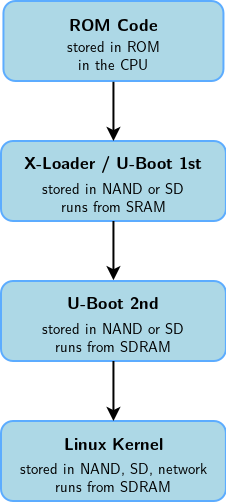
\includegraphics[width=0.2\textwidth]{bootloader-spl.png}
  \caption{Most common boot process from power on to the Linux kernel}
\end{figure}

Most commonly, when a board is powered on, the processor loads a small embedded ROM code which will loads a bootloader in the SRAM limited in size. This bootloader, called SPL or Secondary Program Loader, will take care of basic hardware initialization (mainly DRAM) and the loading of a full size bootloader in DRAM with user interaction. This full size bootloader will then be able to starts the Linux kernel in RAM.

\item Root filesystem (rootfs):

The Linux kernel follows the Filesystem Hierarchy Standard\footnote{\url{https://en.wikipedia.org/wiki/Filesystem\_Hierarchy\_Standard}} which states that everything is organized in directories in a tree-like hierarchy and all directories are subdirectories of the "/" (root) directory. Unlike Microsoft Windows which creates drives for each filesystem, the Linux kernel uses a subdirectory of the root directory to mount the filesystem. The root filesystem contains the files needed for booting the system and is required for mounting other filesystems, thus, without a root filesystem, the Linux kernel will never be able to boot.

\item Mainline, upstream:

Refers to the official current version of a software - the Linux kernel for example - being developed. Mainlining or upstreaming is the process of adding code to the software's mainline version - from \url{http://kernel.org} for the Linux kernel. This process includes comments and critics from the community supporting the software and then validation of the proposed code by the developers in charge of the software part impacted by the proposed code. In the Linux kernel, we call these developers maintainers. When the maintainer of a part of the Linux kernel validates a code snippet, it is merged to this part mainline version until it gets added to the Linux kernel mainline version.

\item User space:

The Linux kernel with every tool used to schedule programs or directly interacts with the hardware runs in kernel space. Programs executed by users without privileges are run in user space and uses tools from the kernel space as an abstraction for the hardware communication.

\end{itemize}
